\documentclass{article}

\usepackage[margin=1in]{geometry}
\usepackage{amsmath,amsthm,amssymb}
\usepackage{bbm, enumerate, tikz}

\newenvironment{problem}[2][Problem]{\begin{trivlist}
\item[\hskip \labelsep {\bfseries #1}\hskip \labelsep {\bfseries #2.}]}{\end{trivlist}}
\newenvironment{note}[1][Note.]{\begin{trivlist}
\item[\hskip \labelsep {\bfseries #1}]}{\end{trivlist}}

\begin{document}

\title{Complex Analysis: Homework 13}
\author{Peter Kagey}

\maketitle

% -----------------------------------------------------
% Problem
% -----------------------------------------------------
\begin{problem}{3} (page 206) \\
  The formula (42) permits us to evaluate the \textit{probability integral} \[
    \int_0^\infty e^{-t^2} dt
      = \frac{1}{2} \int_0^\infty e^{-x}x^{-1/2} dx
      = \frac{1}{2} \Gamma(1/2)
      = \frac{1}{2} \sqrt{\pi}
  \]
  Use this result together with Cauchy's theorem to compute the
  \textit{Fresnel integrals} \[
    \int_0^\infty \sin(x^2) dx
    = \int_0^\infty \cos(x^2) dx
    = \frac{1}{2}\sqrt{\pi/2}
  \]
\end{problem}
\begin{proof} \text{} \\
  The plan is to use the construction from Wikipedia and integrate
  $f(z) = e^{-z^2}$ along the contour given by \begin{align}
    \gamma_{R,1} &= \{t + 0i\ |\ x \in [0, R] \} \\
    \gamma_{R,2} &= \{R e^{it}\ |\ t \in [0,\pi/4] \} \\
    \gamma_{R,3} &= \{te^{i\pi/4}\ |\ t \in [0, R]\}.
  \end{align}
  As seen in the following picture:\\
  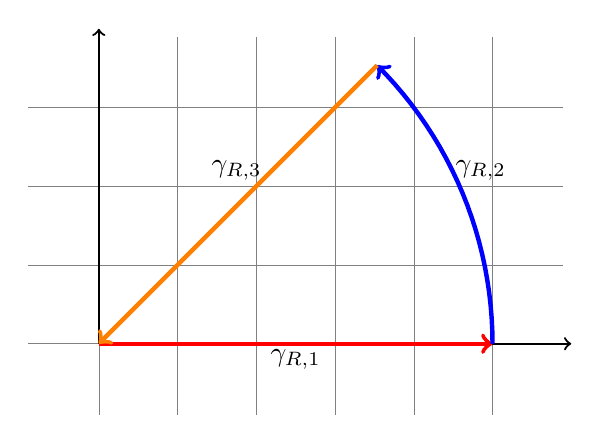
\begin{tikzpicture}
    \draw[very thin,color=gray] (-0.9,-0.9) grid (5.9,3.9);
    \draw[thick, ->] (0,0)--(6,0);
    \draw[thick, ->] (0,0)--(0,4);
    \draw[ultra thick, ->, draw=red, domain=0:5] plot ({\x}, {0});
    \draw node at (2.5, -0.2) {$\gamma_{R,1}$};
    \draw[ultra thick, ->, draw=blue, domain=0:45] plot ({5*cos(\x)}, {5*sin(\x)});
    \draw node at (4.85, 2.2) {$\gamma_{R,2}$};
    \draw[ultra thick, <-, draw=orange, domain=0:5] plot ({\x*cos(45)}, {\x*sin(45)});
    \draw node at (1.75, 2.2) {$\gamma_{R,3}$};
  \end{tikzpicture}
  \\
  The first integral is known: \[
    \lim_{R\rightarrow \infty}\int_{\gamma_{R,1}} f(z)\,dz
      = \int_0^\infty e^{-t^2} dt
      = \frac{1}{2}\sqrt{\pi}.
  \]
  The second integral vanishes in the limit: \begin{align}
    \int_{\gamma_{R,2}} f(z)\,dz
      &= iR\int_0^{\pi/4}\exp(-(Re^{it})^2)\cdot e^{it}\,dt
  \end{align}
  so by looking at the modulus, we get \begin{align}
    \left|\int_{\gamma_{R,2}} f(z)\,dz\right|
    &\leq R\int_0^{\pi/4}|\exp(-R^2e^{2it})| \cdot |e^{it}|\,dt \\
    &= R\int_0^{\pi/4}|e^{-R^2\cos(2t)}|\cdot\underbrace{|e^{-iR^2\sin(2t))}|}_{=1}\,dt \\
    &\leq R\int_0^{\pi/4}|e^{-R^2(\pi/4 - t)}|\,dt \\
    &= \frac{R}{e^{R^2\pi/4}}\int_0^{\pi/4}|e^{R^2t}|\,dt \\
    &= \frac{R}{e^{R^2\pi/4}}\left[\frac{e^{R^2t}}{R^2}\right]_0^{\pi/4} \\
    &= \frac{R}{e^{R^2\pi/4}}\left[\frac{e^{R^2\pi/4}}{R^2} - \frac{1}{R^2}\right] \\
    &= \frac{1}{R} - \frac{1}{Re^{R^2\pi/4}} \\
    &\leq \frac{1}{R}.
  \end{align}
  Thus \[
    \lim_{R \rightarrow \infty}\int_{\gamma_{R,2}} f(z)\,dz = 0.
  \]
  Next, the third integral: \begin{align*}
    \int_{\gamma_{R,3}} f(z)\,dz
      &= \int_R^0 e^{i\pi/4}\exp(-t^2\underbrace{e^{i\pi/2}}_{=i})\,dt \\
      &= e^{i\pi/4}\int_R^0 e^{-it^2}\,dt \\
      &= e^{i\pi/4}\int_R^0 \cos(-t^2) + i \sin(-t^2)\,dt \\
  \end{align*}
  Because $f$ is entire, it follows from Cauchy's theorem that \[
    \int_{\gamma_{R,1}} f(z)\,dz + \int_{\gamma_{R,2}} f(z)\,dz + \int_{\gamma_{R,3}} f(z)\,dz = 0,
  \] including in the limit, therefore \begin{align*}
    \lim_{R\rightarrow \infty}\left(-\int_{\gamma_{R,3}} f(z)\,dz\right)
      &= e^{i\pi/4}\int_0^\infty \cos(-t^2) + i \sin(-t^2)\,dt \\
      &= -\frac{1}{2}\sqrt{\pi}.
  \end{align*} This means that \begin{align}
    \int_0^\infty \cos(-t^2) + i \sin(-t^2)\,dt
    &= \int_0^\infty \cos(t^2) - i \sin(t^2)\,dt \\
    &= \frac{\sqrt{\pi}}{2e^{i\pi/4}} \\
    &= \left(\frac{1}{2} - \frac{i}{2}\right)\sqrt{\frac{\pi}{2}}
  \end{align}
    so by looking at the real and purely imaginary parts it follows that
    \begin{align}
    \int_0^\infty \cos(t^2)\,dt
      = \frac{1}{2}\sqrt{\frac{\pi}{2}}
      = \int_0^\infty \sin(t^2)\,dt.
  \end{align}
\end{proof}
\pagebreak

% -----------------------------------------------------
% Problem
% -----------------------------------------------------
\begin{problem}{2} (page 212) \\
  Assume that $f(z)$ has genus zero so that \[
    f(z) = z^m \prod_n \left(1-\frac{z}{a_n}\right).
  \] Compare $f(z)$ with \[
    g(z) = z^m \prod_n \left(1 - \frac{z}{|a_n|}\right)
  \] and show that the maximum modulus $\displaystyle\max_{|z|=r} |f(z)|$ is
  less than or equal to the maximum modulus of $g$, and the minimum modulus of
  $f$ is greater than or equal to the minimum modulus of $g$.
\end{problem}
\begin{proof} \text{} \\
\end{proof}

\end{document}
